\documentclass[12pt]{article}
\usepackage[top=1in, bottom=1in, left=.75in, right=.75in]{geometry}
\usepackage{amsmath}
%\usepackage[]{enumitem}
\usepackage{enumerate}
\usepackage{fancyhdr}
\usepackage{graphicx, xcolor, setspace, adjustbox}
\usepackage{txfonts}
\usepackage{multicol,coordsys,pgfplots}
\usepackage[scaled=0.86]{helvet}
\renewcommand{\emph}[1]{\textsf{\textbf{#1}}}
\usepackage{anyfontsize}
% \usepackage{times}
% \usepackage[lf]{MinionPro}
\usepackage{tikz,pgfplots}
%\def\degC{{}^\circ{\rm C}}
\def\ra{\rightarrow}
\usetikzlibrary{calc,arrows.meta, shapes, angles, quotes}
\pgfplotsset{compat = newest}
\newcommand{\blank}[1]{\rule{#1}{0.75pt}}

\pgfplotsset{my style/.append style={axis x line=middle, axis y line=
middle, xlabel={$x$}, ylabel={$y$}}}


%\usepackage{draftwatermark}
%\SetWatermarkText{Draft}
%\DraftwatermarkOptions{color={[gray]{.9}}}
%\SetWatermarkScale{1.5}

%axis equal

%yticklabels={,,} , xticklabels={,,}

% \setmainfont{Times}
% \def\sansfont{Lucida Grande Bold}
\parindent 0pt
\parskip 4pt
\pagestyle{fancy}
\fancyfoot[C]{\emph{\thepage}}
\fancyfoot[R]{v1}
\fancyhead[L]{\ifnum \value{page} > 1\relax\emph{Math F251X Calculus I: Final Exam}\fi}
\fancyhead[R]{\ifnum \value{page} > 1\relax\emph{Fall 2023}\fi}
\headheight 15pt
\renewcommand{\headrulewidth}{0pt}
\renewcommand{\footrulewidth}{0pt}
\let\ds\displaystyle
\def\continued{{\emph {Continued....}}}
\def\continuing{{\emph {Problem \arabic{probcount} continued....}}\par\vskip 4pt}


\newcounter{probcount}
\newcounter{subprobcount}
\newcounter{subsubprobcount}
\newcommand{\thesubproblem}{\emph{\alph{subprobcount}.}}
\newcommand{\thesubsubproblem}{\emph{\roman{subsubprobcount}.}}
\def\problem#1{\setcounter{subprobcount}{0}%
\addtocounter{probcount}{1}{\emph{\arabic{probcount}.\hskip 1em(#1)}}\par}
\def\subproblem#1{\par\hangindent=1em\hangafter=0{%
\addtocounter{subprobcount}{1}\thesubproblem\emph{#1}\hskip 1em}}
\def\subsubproblem#1{\par\hangindent=1em\hangafter=0{%
\addtocounter{subsubprobcount}{1}\thesubsubproblem\emph{#1}\hskip 1em}}
\def\probskip{\vskip 10pt}
\def\medprobskip{\vskip 2in}
\def\subprobskip{\vskip 45pt}
\def\bigprobskip{\vskip 4in}


\newenvironment{subproblems}{%
\begin{enumerate}%
\setcounter{enumi}{\value{subprobcount}}%
\renewcommand{\theenumi}{\emph{\alph{enumi}}}}%
{\setcounter{subprobcount}{\value{enumi}}\end{enumerate}}

\newenvironment{subsubproblems}{%
\begin{enumerate}%
\setcounter{enumi}{\value{subsubprobcount}}%
\renewcommand{\theenumi}{\emph{\roman{enumi}}}}%
{\setcounter{subprobcount}{\value{enumi}}\end{enumerate}}


\newcommand{\be}{\begin{enumerate}}
\newcommand{\ee}{\end{enumerate}}


\begin{document}

{\emph{\fontsize{26}{28}\selectfont Fall 2023 \hfill
\hfill Math F251X}}

\begin{center}
{\emph{\fontsize{32}{36}\selectfont Calculus I: Final Exam}}
\end{center}
\vskip 1.cm
\strut\vtop{\halign{\emph#\hskip 0.5em\hfil&#\hbox to 2in{\hrulefill}\cr
\emph{\fontsize{18}{22}\selectfont Name:}&\cr
\noalign{\vskip 10pt}
%\emph{\fontsize{18}{22}\selectfont Student Id:}&\cr
%\noalign{\vskip 10pt}
%\emph{\fontsize{18}{22}\selectfont Calculator Model:}&\cr
}}
\hfill
\vtop{\halign{\emph{\fontsize{18}{22}\selectfont #}\hfil& \emph{\fontsize{18}{22}\selectfont\hskip 0.5ex $\square$ #}\hfil\cr
Section: & 9:15 (Mohamed Nouh)\cr
\noalign{\vskip 4pt}
         & 11:45 (James Gossell)\cr
\noalign{\vskip 4pt}
         & Online (Leah Berman)\cr}}
%
\vfill
{\fontsize{18}{20}\selectfont\emph{Rules:}}

\begin{itemize}
\item Partial credit will be awarded, but you must {\bf show your work}.

\item You may have a single handwritten $3'' \times 5''$ notecard, both sides.

\item Calculators are \emph{not allowed}. 

\item Place a box around your  \fbox{FINAL ANSWER} to each question where appropriate.

\item Turn off anything that might go beep during the exam.

\item You have two hours to complete the exam.

\end{itemize}

%If you need extra space, you can use the back sides of the pages.
%Please make it obvious  when you have done so.

%Good luck!
\vfill
\def\emptybox{\hbox to 2em{\vrule height 16pt depth 8pt width 0pt\hfil}}
\def\tline{\noalign{\hrule}}
\centerline{\vbox{\offinterlineskip
{
\bf\sf\fontsize{18pt}{22pt}\selectfont
\hrule
\halign{
\vrule#&\strut\quad\hfil#\hfil\quad&\vrule#&\quad\hfil#\hfil\quad
&\vrule#&\quad\hfil#\hfil\quad&\vrule#\cr
height 3pt&\omit&&\omit&&\omit&\cr
&Problem&&Possible&&Score&\cr\tline
height 3pt&\omit&&\omit&&\omit&\cr
&1&&8&&\emptybox&\cr\tline
&2&&8&&\emptybox&\cr\tline
&3&&10&&\emptybox&\cr\tline
&4&&7&&\emptybox&\cr\tline
&5&&7&&\emptybox&\cr\tline
&6&&15&&\emptybox&\cr\tline
&7&&10&&\emptybox&\cr\tline
&8&&6&&\emptybox&\cr\tline
&9&&8&&\emptybox&\cr\tline 
&10&&11&&\emptybox&\cr\tline 
&11&&10&&\emptybox&\cr\tline \tline 
&Extra Credit&&(5)&&\emptybox&\cr\tline \hline
&Total&&100&&\emptybox&\cr
}\hrule}}}

\newpage
%\begin{enumerate}
%%%%





%%%%%%%%%%%%%%%%% Compute some integrals
\problem{8 points} Compute the following \emph{indefinite integrals}. Show your work. Clearly indicate any substitutions you use in such a way that someone else can follow your work.

\begin{subproblems}
%\item $\displaystyle{\int ( e^{-x} + 5^{2x+1}) dx}$
\item $\displaystyle{\int \left( \sin(2x) + e^{x} - \frac{\sqrt[3]{x}}{6} +\frac{1}{\sqrt{1-x^{2}}} \right) \ dx}$

\vfill

\item $\displaystyle{\int \frac{\ln(2x+1)}{4x+2}\ dx}$ 

\vfill

%\item $\displaystyle{\int \frac{4}{x^2 +6x + 13} dx}$ Too hard. None of my students can complete a dsquare.
%
%\vfill


\end{subproblems}

%%%%%%%%%%% 
\problem{8 points} Compute the following \emph{limits}. Show your work clearly. Make sure you use \emph{limit notation} where required; an answer that does not use proper notation will not receive full credit. Use = to show things are equal. If you use L'H\^opital's rule, write $\stackrel{H}{=}$ or  $\stackrel{L'H}{=}$ to indicate where you are applying it.

\begin{subproblems}
\item $\ds{\lim_{x\to \infty} \frac{6x^{4} - 5x^2}{7x^{4} - 14}}$ 
\vfill

%\item $\ds{\lim_{t \to 0} \frac{3^{t} -1}{t^4- t}}$ %%just DS

%\vfill

%\item $\ds{\lim_{x\to - \infty} \frac{x^3}{e^x}}$
%%%%%%%% I wanted a really standard one where they just need to factor and cancel.
\item $\ds{\lim_{x\to 3} \frac{2 x^2 - 5x - 3}{x^{2}- 9}}$
\vfill

\end{subproblems}
\newpage

%%%%%% 
%%%%%%%%% Graphical stuff
\problem{10 points} Consider the graph of the function $f(x)$ shown below:
	\vspace{-.5cm}
	\begin{center}
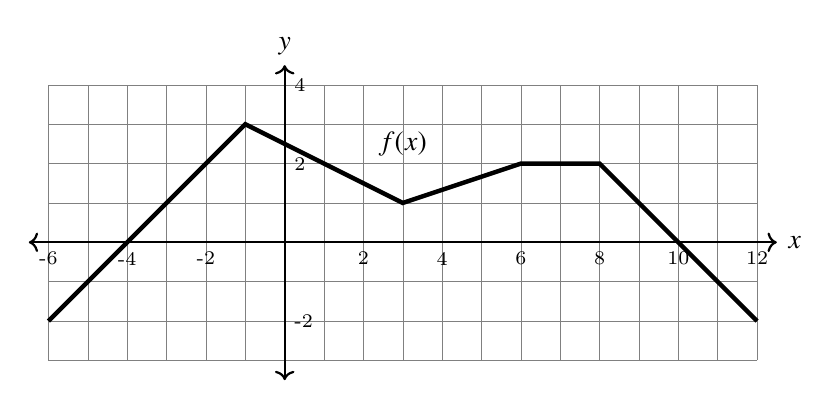
\begin{tikzpicture}[scale = .5]
%cubic
%\begin{axis}[xscale = 1, yscale = 1, thick, my style, xtick={-2,2,4,...,10}, ytick={-1,1,2,3,4},xmin=-5, xmax=10, ymin=-5, ymax=6, minor y tick num=1, minor x tick num=1, 
%mark size=3.0pt, grid = major, ]
%%\addplot[ultra thick, -,domain=-4:-2, samples=100, <-]coordinates {(-4,-2)(-2,2)};
%\addplot[ultra thick, domain=-5:5, samples=100, ,]{sqrt(25-x^2)};
%\addplot[ultra thick, ->,domain=5:9, samples=100]{-1/2*(x-5)};
%\end{axis}

\draw[help lines] (-6, -3) grid (12, 4);
\draw[thick,<->] (-6.5,0) -- (12.5,0) node[right] {$x$};
\draw[thick,<->] (0,-3.5) -- (0,4.5) node[above] {$y$};
%\draw[ultra thick] (5,0) -- (11,-3);
\draw[ultra thick] (-6, -2) -- (-1,3) -- (3,1) -- (6,2) -- (8,2) -- (12,-2);
%\draw[ultra thick] (5,0) arc (0:180:5);
\foreach \i in {-6, -4,-2,2,4,6,8,10, 12} {\path  (\i,0)node[below, font = \scriptsize] {\i};}
\foreach \i in {-2,2,4} {\path  (0, \i)node[right, font = \scriptsize] {\i};}
\node at (3,2.5) {$f(x)$};
\end{tikzpicture}
\end{center}

\begin{subproblems}
\item Compute $\ds{\int_{3}^{11}f(x) \ dx}$.

\vfill


\item  Let $\ds{F(t) = \int_{-6}^{t} f(x) \ dx}$. 
\emph{On the interval} $[-6, 3]$, at what $t$-value does $F(t)$ have an absolute maximum? Where does it have an absolute minumum? 

\smallskip

\begin{itemize}
%\begin{enumerate}[font = \sffamily,label=\textbf{\roman*}.]
	
\item $F(t)$ has a maximum at $t = $ \blank{2cm} %because %\hrulefill. 

\medskip

\item $F(t)$ has a minimum at $t = $ \blank{2cm} %because %\hrulefill. 

%\end{enumerate}
\end{itemize}

\bigskip

\item Determine $f'(1) = \blank{2cm}$

\bigskip

\item What can you say about $\ds\lim_{x \to -1} f'(x)$? (Note that's asking for the limit of the derivative, not the function.) Explain your answer. 

\vfill
\end{subproblems}

\newpage

%%%%%%%%%%%%%%%%% optimization
%\problem{?? points} 
%\begin{minipage}[b]{.6\linewidth}A rectangular storage container with an open top needs to have a volume of $V = 30 \: \textrm{m}^3$. The length $y$ of its base is twice its width $x$. Material for the base costs $ \$ 10$ per $\textrm{m}^{2}$. Material for each of the sides costs $ \$ 5$ per $\textrm{m}^{2}$. 
%\end{minipage}
%%
%\hfill
%%
%\begin{minipage}[b]{.3\linewidth}
%%
%\begin{tikzpicture}[side/.style = { black,thick , fill=gray!50, , fill opacity = .3}, scale = 1.2]
%\pgfmathsetmacro{\cubex}{2} %x width 
%\pgfmathsetmacro{\cubey}{1.2} %z height
%\pgfmathsetmacro{\cubez}{1} %y length
%\draw[side, fill opacity = 1] (0,0,0) -- ++(-\cubex,0,0) -- ++(0,-\cubey,0) -- ++(\cubex,0,0) -- cycle;
%\draw[side, fill opacity = 1] (0,0,0) -- ++(0,0,-\cubez) -- ++(0,-\cubey,0) -- ++(0,0,\cubez) -- cycle;
%
%\draw[side] (-\cubex, -\cubey,-\cubez) -- ++(\cubex,0,0) -- ++(0,\cubey,0) -- ++(-\cubex,0,0) -- cycle;
%\draw[side] (-\cubex, -\cubey,-\cubez) -- ++(0,0,\cubez) -- ++(0,\cubey,0) -- ++(0,0,-\cubez) -- cycle;
%\draw[side,fill=black!80, opacity = .6] (-\cubex, -\cubey,-\cubez) -- ++(\cubex,0,0) -- ++(0,0,\cubez) -- ++(-\cubex,0,0) -- cycle;
%
%\draw[|-|] (-\cubex-.2,0,0)-- node[left]{$z$} +(0, -\cubey, 0);
%\draw[|-|] (0,-\cubey-.2,0)-- node[below]{$y$} +(-\cubex, 0, 0);
%\draw[|-|] (.2,-\cubey-.1,0)-- node[below right]{$x$} +(0, 0, -\cubez);
%%\draw 
%%\path  (-\cubex, -\cubey,-\cubez) node[draw, circle, red]{};
%%\path (0,0,0) node[draw, circle, black]  {};
%%\path (0,-\cubey,0) node[draw, circle, green]  {y};
%%\path (-\cubex,0,0) node[draw, circle, blue]  {x};
%%\path (0,0,-\cubez) node[draw, circle, orange]  {z};
%
%
%\end{tikzpicture}
%
%\end{minipage} 
%
%\begin{subproblems}
%
%\item Write a function, in terms of $x$, that gives the total cost of the container.
%
%\vspace{1.5in}
%
%\item Find the value of $x$ that \emph{minimizes} the cost of the container.
%\vfill
%
%\item %\emph{How much} does the cheapest container cost, and what are its \emph{dimensions}? Answer the question with a sentence.%
%Find the cost of the material for the cheapest container. Write your answer in a sentence.
%
%\vspace{1in} 
%
%\end{subproblems}


%POSSIBLE OTHER PROBLEMS
%
%\#1 


%Find the equation of the tangent line to the curve ${y^{2}=4x^{3}+8x^{2}-12x}$ at the point $(-1,4)$.
\problem{7 points} A portion of the implicitly defined curve
$ 3 + xy^{2} = x^{3}$
is shown below. 

\begin{subproblems}
%\begin{minipage}[t]{.6\linewidth}

%\vspace{0pt}

\item Determine $\ds \frac{dy}{dx}$.

%\vfill
%\vfill
%\end{minipage}
\hfill
%\begin{minipage}[t]{.4\linewidth}
%\begin{center}
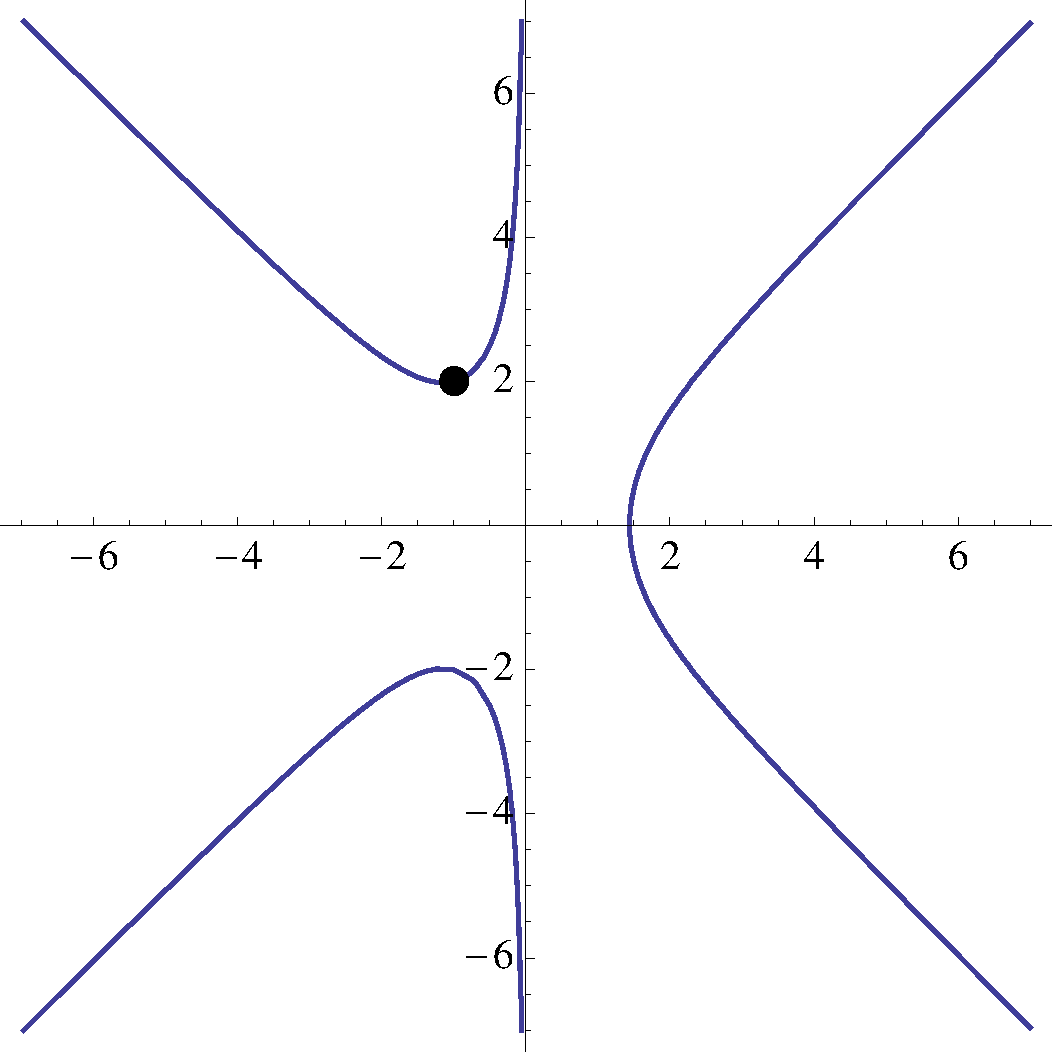
\includegraphics[width=.3\linewidth]{ImpDifPlot}
%\end{center}
%\end{minipage}


%\Part Find the slope of the tangent line to the curve at the point $(-1,2)$ (shown as the black dot). Please give an exact answer, not a decimal approximation. 

\item \emph{Write the equation} of the tangent line to the curve at the point $(-1,2)$, which is shown with a black dot on the curve. \emph{Clearly draw and label} the tangent line on the graph. %(Check: does it agree with your equation?)
\vfill
\vfill

\end{subproblems}
%\newpage


\problem{7 points} \begin{minipage}{.7\linewidth}Suppose a rectangular box has two square sides and four sides where the length of the side is two times the width of the side (see diagram).

Suppose the short side of the box is measured to be 10 cm $\pm$ 1 mm (1mm =  1/10 cm), and the volume is computed. Use linearization or differentials to determine the \emph{error} in the measurement of the volume.  Write your answer with a sentence, using correct units.\end{minipage}
    \hspace{1cm}
\begin{minipage}{.3\linewidth}
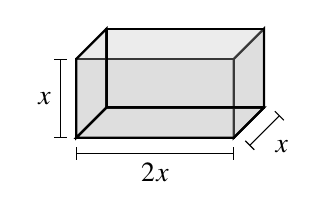
\begin{tikzpicture}[side/.style = { black,thick , fill=gray!50, , fill opacity = .3}, scale = 1.0]
\pgfmathsetmacro{\cubex}{2} %x width 
\pgfmathsetmacro{\cubey}{1} %z height
\pgfmathsetmacro{\cubez}{1} %y length
\draw[side, ] (0,0,0) -- ++(-\cubex,0,0) -- ++(0,-\cubey,0) -- ++(\cubex,0,0) -- cycle;
\draw[side,] (0,0,0) -- ++(0,0,-\cubez) -- ++(0,-\cubey,0) -- ++(0,0,\cubez) -- cycle;

\draw[side] (-\cubex, -\cubey,-\cubez) -- ++(\cubex,0,0) -- ++(0,\cubey,0) -- ++(-\cubex,0,0) -- cycle;
\draw[side] (-\cubex, -\cubey,-\cubez) -- ++(0,0,\cubez) -- ++(0,\cubey,0) -- ++(0,0,-\cubez) -- cycle;
\draw[side,%fill=black!80, opacity = .6
] (-\cubex, -\cubey,-\cubez) -- ++(\cubex,0,0) -- ++(0,0,\cubez) -- ++(-\cubex,0,0) -- cycle;

\draw[|-|] (-\cubex-.2,0,0)-- node[left]{$x$} +(0, -\cubey, 0);
\draw[|-|] (0,-\cubey-.2,0)-- node[below]{$2x$} +(-\cubex, 0, 0);
\draw[|-|] (.2,-\cubey-.1,0)-- node[below right]{$x$} +(0, 0, -\cubez);
%\draw 
%\path  (-\cubex, -\cubey,-\cubez) node[draw, circle, red]{};
%\path (0,0,0) node[draw, circle, black]  {};
%\path (0,-\cubey,0) node[draw, circle, green]  {y};
%\path (-\cubex,0,0) node[draw, circle, blue]  {x};
%\path (0,0,-\cubez) node[draw, circle, orange]  {z};


\end{tikzpicture}
\end{minipage}


\vfill

\vfill

\vfill

%(ii) Determine the \emph{percent} error in the computation?

\newpage

%%%%%%%%%%%%%%%%%%%%
\problem{15 points} A hot air balloon rises with an upward velocity of $\displaystyle{ v(t)=2te^{-t^2} = \frac{2t}{e^{t^{2}}}}$ kilometers per minute (km/min),  $t$ minutes after it is launched ($t \ge 0$).
\begin{subproblems}
%	\item What is the balloon's initial velocity, $v(0)$? Include units in your answer.
%	\vfill
	\item What is the balloon's \emph{initial acceleration}, $a(0)$? Include units in your answer.
	\vspace{1in}
	\item At what \emph{time} does the balloon reach its \emph{maximum upward velocity}? Use calculus techniques to \emph{verify} that the time you find really is where the velocity is a maximum. Include units in your answer, and show your work.
	\vfill
	\vfill
	\vfill
	\item \emph{Evaluate} the integral $\displaystyle \int_0^2 v(t)\ dt$. Show your work and simplify your answer as much as possible.
	\vfill
		\item \emph{Write a sentence} explaining the meaning of your answer to the previous part in the context of the problem, in a way someone who has not taken calculus can understand. Include units in your answer.
	\vspace{1cm}
\end{subproblems}

\newpage

%%%%%%%%%%%%%%%% Related Rates

\problem{10 points} A rocket is launched vertically off of a launch pad. A camera is positioned $5$ kilometers from the launch pad. When the rocket is $12$ kilometers above the launch pad, its velocity is $2$ km/sec. (See the diagram below.)\\

%\includegraphics[scale=0.8]{RocketPicture}

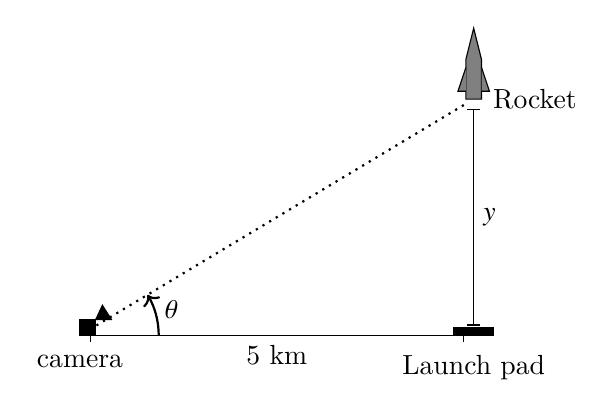
\begin{tikzpicture}
\pgfmathsetmacro{\cam}{.2}
\draw[fill=black] (0,0) rectangle (\cam,\cam);
\draw [fill = black] (\cam,\cam) -- +(0:.2)-- +(65:.2) -- (\cam, \cam);
\node[label=below:{camera}] (b) at (0,0){};
\node[label=below:{Launch pad}] (a) at (5,0){};
\draw[fill=black] ($(a)-({(2.5*\cam)/2},0)$) rectangle ($(a) + ({(2.5*\cam)/2},\cam/2)$);
\node[label=right:{Rocket}] (c) at (5,3){};

\draw[|-|] (b) -- node[midway, below]{5 km} (a);
\draw[|-|] (a) -- node[midway, right]{$y$} (c);
%\draw[-latex] (1,0) arc[start angle=0, end angle={atan(5/3)},radius=12 pt] node[midway,right] {$\theta$} ;
\draw[dotted, thick] (b) -- (c);
%\draw (0:0:0.5) arc (120:{atan(8/5)}:0.5) ;
\draw pic["$\theta$",draw=black, thick,->,angle eccentricity=1.2,angle radius=1cm] {angle=a--b--c};
\coordinate (T) at ($(c) + (\cam/2,{3*\cam - \cam/2})$){};
\coordinate (T2) at ($(c) + (-\cam/2,{3*\cam - \cam/2})$){};
\coordinate (T3) at ($(c) + (-\cam/2,0)$){};
\coordinate (T4) at ($(c) + (\cam/2,0)$){};
\coordinate (T5) at ($(c) + (0, 4.5*\cam)$){};

%\node[draw, circle, blue] (c){};

%\path (T) node[draw, circle, inner sep = 1 pt]{};
%\path (T2) node[draw, red,circle, inner sep = 1 pt]{};
%\path (T3) node[draw,blue,  circle, inner sep = 1 pt]{};
%\path (T4) node[draw,green,  circle, inner sep = 1 pt]{};
%\path (T5) node[draw, circle, inner sep = 1 pt]{};

\draw[fill = gray] (T) -- (T5) -- (T2) -- (T3) -- (T4) -- cycle;

\draw[fill = gray] ($(T4)!.2!(T)$) -- +(.1, 0) -- ($(T4)!.8!(T)$);
\draw[fill = gray] ($(T3)!.2!(T2)$) -- +(-.1, 0) -- ($(T3)!.8!(T2)$);



%\draw[fill = gray] ($(c) - (\cam/2,0)$) -- +(\cam,0) -- +(0,3*\cam) -- +(90:\cam) -- +(180:\cam) -- cycle;
%\draw[fill = gray] ($(c) - (\cam/2,\cam)$) rectangle  (T);
%\draw[fill = gray] (t) -- ($(c) + (0,2)$) -- (t2) -- (t);
%\node[draw, red, inner sep = 2 pt, circle] (T){};
\end{tikzpicture}

Find the necessary \emph{rate of change} of the camera's angle $\theta$ so that it stays focused on the rocket at the instant when the rocket is $12$ kilometers above the launch pad. Answer the question with a \emph{sentence}, including correct units.


\newpage


%%%%%%%%% Interp infinite limit etc.
\problem{6 points} The population of rabbits in a local park, measured since 2011, can be modeled by the equation 
\[ P(t) = \frac{10\, 000 e^{t/10}}{480 + 20 e^{t/10}}\]
where $t$ measures time, in years, since 2011.

\begin{subproblems}
\item How many rabbits were in the park in 2011? Simplify your answer.
\vspace{1.5cm}


\item \emph{Compute} $\ds \lim_{t \to \infty} P(t)$. Show your work clearly, with correct use of notation. 

\vfill


\item  \emph{Write a sentence} that explains the meaning of the limit you just calculated, in terms a person who has not taken calculus can understand. 

\vspace{1.5cm}

\end{subproblems}

%%%%%%%% 
\problem{8 points} Compute the following \emph{derivatives}. Show your work. You do NOT need to simplify your answer.


\begin{subproblems}

\item $\displaystyle{ f(x) = \sqrt{x}\left(\ln(x^3-x^2)\right)}$

%$f'(x) = $
\vfill 

\item $\displaystyle{ g(x) = \left(e^{-x} + \frac{\arctan(x)}{2}\right)^5}$. (Note $\arctan(x) = \tan^{-1}(x)$.)

%$g'(x) = $
\vfill 

\end{subproblems}


\newpage

%%%%%%%%%%%%%%% curve sketching
\problem{11 points} \emph{Sketch} a graph of a function $h(x)$ that satisfies all of the following properties. 

After drawing the graph:

\begin{itemize}
\item \emph{Label} on the graph the following things, if they exist, by drawing a point on the graph and labeling: any local maximums by writing  \textsf{LOCAL MAX}, local minimums by writing \textsf{LOCAL MIN}, inflection points by writing \textsf{IP} 
\item \emph{Draw} any horizontal and vertical asymptotes with dashed lines and \emph{label} them with their equation.
\item \emph{Mark} any important $x$-values and $y$-values (with numbers) on the $x$- and $y$-axes.
\end{itemize}


\emph{Properties:}
\begin{multicols}{2}
\begin{itemize}
\item The domain of $h(x)$ is $(-\infty, 5)$
\item $h(0)=0$ and $h(2)=-3$
\item $h'(x) < 0$ on the interval $(-\infty, 2)$
\item $h'(x) > 0$ on the interval $(2,5)$
\columnbreak
\item $h''(x) < 0$ on the interval $(-\infty, 0)$
\item $h''(x) > 0$ on the interval $(0,5)$
\item $\ds \lim_{x \to -\infty} h(x) = 3$
\item $\ds \lim_{x \to 5^-} h(x) = +\infty$
\end{itemize}
\end{multicols}

\begin{tikzpicture}
\draw[<->] (-8,0) --  (8,0);
\draw[<->] (0,4) -- (0,-4);
\end{tikzpicture}


\newpage




%%%%%%%%% Interp function
\problem{10 points}A hot cup of coffee in a room whose ambient temperature is $68^{\circ}$F is changing temperature at a rate of $R(t)$, where $t$ is measured in minutes and $R(t)$ is measured in $^{\circ}$F/minute. 

\begin{subproblems}
\item Write down a complete sentence carefully explaining the meaning of $R(5) = -9$ in the context of the problem. Use units in your answer.

\vfill

\item Would you expect $R(t)>0$ or $R(t) <0$? Explain your answer in a sentence, given the context of the problem.

\vfill


\item Write a complete sentence explaining the meaning of the quantity \[\ds \int_{0}^{8} R(t) \ dt = -107\] in the context of the problem. Include units in your answer.

\vfill

\item Assume the cup of coffee started at $200^{\circ}$F and was left sitting on the kitchen counter, untouched. Write an expression that you would need to compute to determine the temperature of the coffee an hour later.

\vfill

\end{subproblems}

\newpage


%\end{enumerate}
%%%%%%%%%%%%%%%%%%%%%%%%%%%

\newpage

%% Extra Credit Newton's Method
\fbox{\emph{Extra Credit}} (5 points) A portion of the graph of the function $f(x)=-\frac{4}{5}x^5+x+\frac{2}{5}\:$ is shown below.

	\begin{tikzpicture}[yscale=1.8,xscale=3.2]
\draw[->] (-0.5,0) -- (2.2,0) node[right] {$x$};
\draw[->] (0,-1.2) -- (0,2.2) node[above] {$f(x)$};
\draw[help lines, dashed] (-0,-1) grid (2,2);
\foreach \x in {1,2}
\draw (\x,-0.1) node[below] {$\x$};
\foreach \y in {1,2}
\draw (-0.1,\y) node[left] {$\y$};
%\draw[scale=0.5, domain=-3:3, smooth, variable=\x, blue] plot ({\x}, {\x*\x});
	\draw[domain=-0.5:1.3, -, ultra thick,smooth, variable=\x] plot({\x},{-0.8*\x^5+\x+0.4});
	\end{tikzpicture}

\begin{enumerate}[a.]%[font = \sffamily,label=\textbf{\alph*}.]
	\item Suppose Newton's method is used to find an approximate solution to
	$f(x)=0$ from an initial guess of $x_1=1$. \emph{Sketch} on the graph how the
	next approximation $x_2$ will be found, \emph{labeling}
	its location on the $x$-axis.
	%\vfill
	\item If your starting guess is $x_1=1$, \emph{compute} $x_2$. 	\vfill
\end{enumerate}

\newpage



\end{document}

%%%%ENDDOCUMENT


